\documentclass[ignoreonframetext,unicode]{beamer}

\usepackage[utf8]{inputenc}
\usepackage[T1]{fontenc}
\usepackage[english,russian]{babel}
\usepackage{amsmath}
\usepackage{amsfonts}
\usepackage{amssymb}
\usepackage{graphicx,pgf}
\usepackage{multimedia}

\usetheme{Warsaw}

\useinnertheme{circles}   %внутренняя тема
%\useoutertheme{smoothbars}   %внешняя тема
\usecolortheme{seahorse}     %цветовая схема
%\usefonttheme{serif}    %шрифты
%\defbeamertemplate*{footline}{shadow theme}
%\setbeameroption{hide notes}

%номера слайдов
\newcommand*\oldmacro{}%
\let\oldmacro\insertshorttitle%
\renewcommand*\insertshorttitle{%
	\oldmacro\hfill%
	\insertframenumber\,/\,\inserttotalframenumber}
\RequirePackage{caption}
\DeclareCaptionLabelSeparator{defffis}{ }
\captionsetup{justification=centering,labelsep=defffis}

%\title{Курсовая работа}
%\subtitle{Численные схемы для аппроксимации неограниченных решений при моделировании обтекания профиля крыла в вихревых методах}
\title[Уравнение изгиба балки]{Нахождение уравнения изгиба балки}
\author[Пиневич В.\,Г.]{Докладчик: Пиневич В.\,Г.\and\\[0.5mm] Научный руководитель: Чередниченко А.\,В.}

\institute[каф. Прикладная математика ФН-2]{группа ФН2-41Б}
\date{\today}
\titlegraphic{
\includegraphics[width=2cm]{logo.png}}
%\renewcommand{\vec}[1]{\text{\mathversion{bold}${#1}$}}


\begin{document}
	
	\begin{frame}[plain]
		\maketitle
		%\insertshortinstitute{Группа ФН2-41Б}
	\end{frame}

	\begin{frame}{Постановка задачи}
		\begin{columns}
			\column{\textwidth}`
			\begin{block}{Условия равновесия}\vspace*{-3.5mm}
			 \[
			 	\begin{cases}
			 	\sum\limits {{F_z = 0}} \\
			 	\sum\limits {{M_z = 0}}
			 \end{cases}
			 \Leftrightarrow
			 \begin{cases}
			 	P + q dz - P - dP = 0 \\
			 	M + P dz + q dz \frac {dz}{z} - M -dM = 0
			 \end{cases}
			 \]
			\end{block}
		\begin{columns}
			\column{0.5\textwidth}
			\begin{block}{Кривизна изогнутого стержня}	
				\[
				\frac{1}{\rho} = \frac{y''}{(1 + y'^2)^{\frac{3}{2}}} \approx y''
				\]
			\end{block}
			\column{0.5\textwidth}\vspace*{-1.0mm}
			\begin{block}{Связь кривизны и момента}	
				\[
				\frac{1}{\rho} = \frac{M}{E J_{x}}
				\]
			\end{block}
		\end{columns}

		\begin{columns}
			\column{0.5\textwidth}
			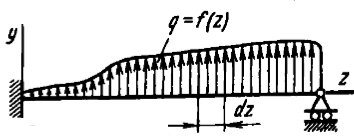
\includegraphics[width=\textwidth]{pic.1.1}
			\column{0.5\textwidth}
			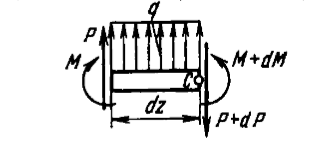
\includegraphics[width=\textwidth]{pic.1.2}
		\end{columns}

		\end{columns}
		
	\end{frame}

	\begin{frame}{Уравнения равновесия стержня и граничные условия}
	
	\begin{columns}
		\column{0.5\textwidth}
			\begin{block}{}	
			\[
			\begin{cases}
				\frac{d P}{d z} = q(z) \\
				\frac {d M}{d z} = P \\
				\frac{d \theta}{d z} = \frac{M}{E J_{x}}\\
				\frac{d y}{d z} = \theta 
			\end{cases}
			\]
		\end{block}
		\column{0.5\textwidth}
		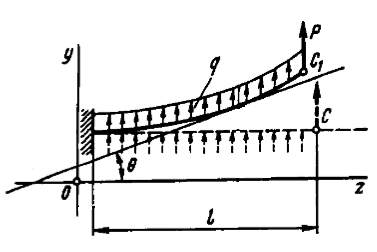
\includegraphics[width=\textwidth]{pic.6}
	\end{columns}

	\begin{columns}
		\column{0.5\textwidth}
		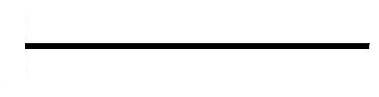
\includegraphics[width=\textwidth]{free}
		\vspace*{-5.5mm}
		\column{0.5\textwidth}
		
		\[
		\begin{cases}
			M = 0\\
			P = 0
		\end{cases}
		\]
	\end{columns}
	
	\begin{columns}
		\column{0.5\textwidth}
		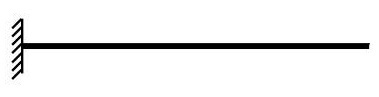
\includegraphics[width=\textwidth]{console}
		\vspace*{-5.5mm}
		\column{0.5\textwidth}
		\[
		\begin{cases}
			y = 0\\
			\theta = 0
		\end{cases}
		\hspace{1.5mm}
		\]
	\end{columns}
	
	\begin{columns}
		\column{0.5\textwidth}
		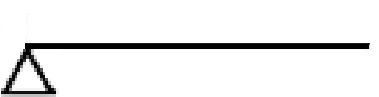
\includegraphics[width=\textwidth]{op}
		\vspace*{-5.5mm}
		\column{0.5\textwidth}
		\[
		\begin{cases}
			y = 0\\
			M = 0
		\end{cases}
		\]
	\end{columns}
		
	\end{frame}

	\begin{frame}{Обобщенные функции Дирака и Хевисайда}	
		
		\begin{columns}
			\column{0.5\textwidth}
					\begin{block}{Функция Дирака}	
				\[
				\delta (z - a) = 
				\begin{cases}
					\infty, z = a \\
					0, z \neq  a	
				\end{cases}
				\]
			\end{block}
			\column{0.5\textwidth}
			\begin{block}{Функция Хевисайда}	
				\[
				H(z - a) = 
				\begin{cases}
					0, z < a \\
					1, z \geqslant a	
				\end{cases}
				\]
			\end{block}
		\end{columns}
		
		\begin{columns}
			\column{0.4\textwidth}
			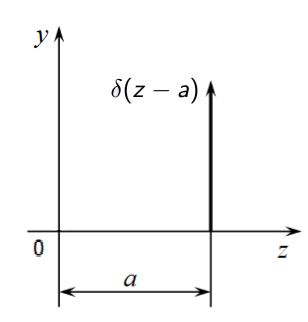
\includegraphics[width=\textwidth]{dirac}
			\column{0.4\textwidth}
			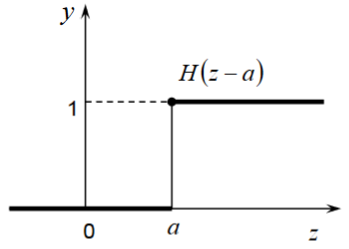
\includegraphics[width=1\textwidth]{heavi}
		\end{columns}
				
		\begin{gather*}
			\int_{b}^z \delta(t - a) d t = H(z - a)
		\end{gather*}
	
	\end{frame}

\begin{frame}{Интегрирование функции Хевисайда}
	
	
		\begin{gather*}
			\mbox{1. } \int_b^z f(t) H(t - a) d t = H(z - a)\int_b^z f(t) d t \hspace{20mm}
		\end{gather*}
		
		
		\begin{gather*}
			\mbox{2. } \int_b^z H(t - a) \int_b^{t} f(t_1) d{t_1} dt = H(z - a) \int_b^z \int_b^{t} f(t_1) d{t_1} dt
		\end{gather*}
		
	

	\begin{columns}
	\column{0.5\textwidth}
	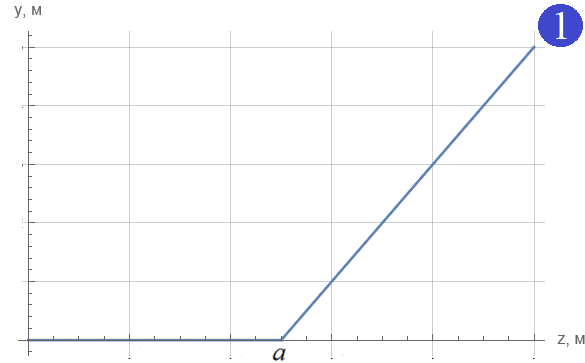
\includegraphics[width=\textwidth]{intHeav}%
	\column{0.5\textwidth}
	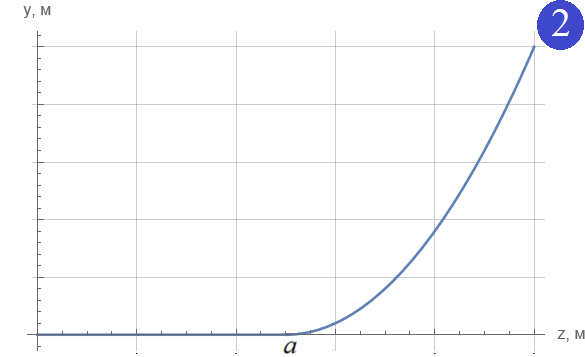
\includegraphics[width=\textwidth]{int2Heav}%
	\end{columns}
	
\end{frame}	

	\begin{frame}{}
	
	\begin{columns}
		\column{0.5\textwidth}
		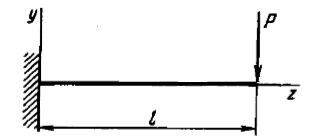
\includegraphics[width=\textwidth]{pic.7}
		\column{0.5\textwidth}
		\vspace*{-2.0mm}
		\begin{block}{Дано}
			$P = 1$ Н \\ 
			$E = 70$~ГПа\\
			$J_{x} = 8,33333 \cdot 10^{-6}$~$\mbox{кг} \cdot \mbox{м}^2$
		\end{block}
	\end{columns}
	\vspace*{-2.0mm}
	\begin{block}{Граничные условия}\vspace*{-1.0mm}
	\[
	\begin{cases}
			y = 0; y'' = 0\mbox{, при } z = 0\\
			y'' = 0; E J_{x} y''' = P\mbox{, при } z = L
	\end{cases}
	\]		
	\end{block}

		\begin{enumerate}
		\item Найдем момент $M = -\int P d z = P(L - z)$
		
		\item Дважды интегрируем, получаем уравнение изгиба балки:
		\vspace*{-2.0mm}
		\begin{gather*}\vspace*{-2.0mm}
			y = \frac{P}{E J_{x}} \int \left(\frac{z^2}{2} - L z + c_1\right) d z = \frac{P}{E J_{x}} \left(\frac{z^3}{6} - \frac{z^2 L}{2} + c_1 z + c_2\right)
		\end{gather*}
		\vspace*{-3.0mm}
		\begin{block}{Итоговое уравнение}\vspace*{-1.0mm}
			\[
			y = \frac{P}{E J_{x}} \left(\frac{z^3}{6} - \frac{z^2 L}{2}\right)
			\]
		\end{block}
		
	\end{enumerate}
	
	\end{frame}

	\begin{frame}{Решение методом обобщенных функций}
	
	\begin{block}{Граничные условия}\vspace*{-1.0mm}
	\[
	\begin{cases}
		y = 0; \theta = 0\mbox{, при } z = 0\\
		y'' = 0; E J_{x} y''' = 0\mbox{, при } z = L
	\end{cases}
	\]		
	\end{block}
	
	\begin{enumerate}
		\item С~помощью~функции~Дирака~запишем:~$E J_{x} y^{IV} = -P \delta (z - L)$
		
		\item Интегрируем:
		$
			E J_{x} y''' = -P H (z - L) + c_1
		$
		
		\item Еще раз интегрируем:
		$
			E J_{x}P \int  (1 - H (z - L)) dz = Pz + c_2
		$
		
		\item Найдем угол поворота балки:
		\begin{gather*}
			E J_{x} y' = P \int (z - L) dz = P \left(\frac{z^2}{2} - L z\right) + c_3
		\end{gather*}
	
	\item Получаем уравнение гибкого изгиба балки:
	\begin{gather*}
		y = \frac{P}{E J_{x}} \left(\frac{z^3}{6} - \frac{z^2 L}{2}\right) + c_3 z + c_4.
	\end{gather*}
		
	\end{enumerate}
\end{frame}

\begin{frame}{Решение задачи}
	\begin{block}{Итоговое уравнение}	
		\[
		y = \frac{P}{E J_{x}} \left(\frac{z^3}{6} - \frac{z^2  L}{2}\right)
		\]
	\end{block}

		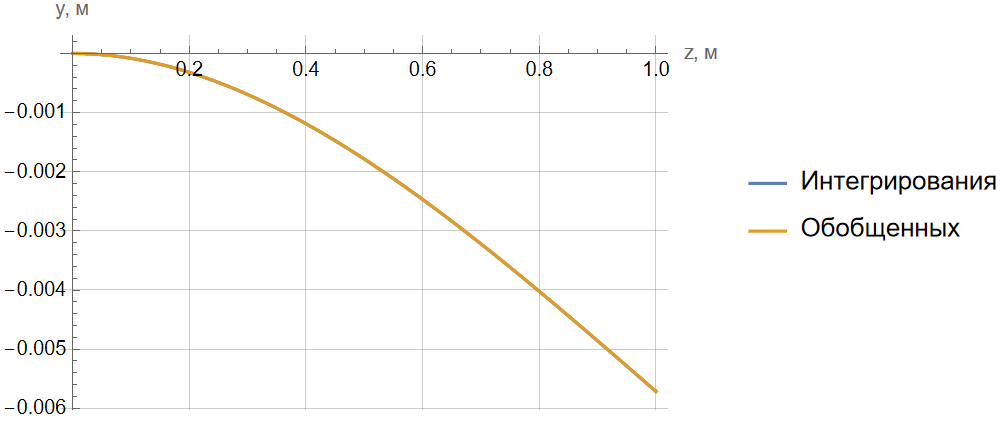
\includegraphics[width=1\textwidth]{g.1}

\end{frame}

	\begin{frame}{Двух опорная балка}
	\begin{columns}
	\column{0.5\textwidth}
	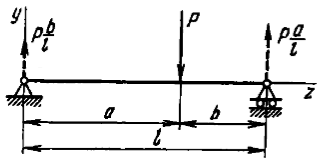
\includegraphics[width=\textwidth]{pic.8}
	\column{0.5\textwidth}
	\begin{block}{Дано}
		$P = 1$ Н \\ 
		$E = 70$~ГПа\\
		$J_{x} = 8,33333 \cdot 10^{-6}$~$\mbox{кг} \cdot \mbox{м}^2$
	\end{block}
	\end{columns}

	\begin{block}{Граничные условия}
	\[
	\begin{cases}
		y_1 = 0 \mbox{, при } z = 0\\
		y_2 = 0 \mbox{, при } z = L\\
		y_1 = y_2 \mbox{ и } y_1' = y_2' \mbox{, при } z = a
	\end{cases}
	\]		
\end{block}

\begin{enumerate}
	\item  Сила $P_1 = \frac{P b}{L} $.
	
	\item 	Четырежды интегрируем, получаем уравнение изгиба $y_1$:
	\begin{gather*}
		y_1 = \frac{P b}{E J_{x} L} \left(\frac{z^3}{6} + c_1^1 z + c_2^1\right)
	\end{gather*}		
\end{enumerate}
	
\end{frame}

\begin{frame}{}
	Рассмотрим вторую часть стержня. 
	\begin{enumerate}
		\item Сила $P_2 = \frac{P a}{L}$.

		\item Четырежды интегрируем, получаем уравнение изгиба  $y_2$: 
		\begin{gather*}
			y_2 = - \frac{P a}{E J_{x} L} \left(\frac{z^3}{6} + \frac{z^2 L}{2} - c_1^2 z + c_2^2\right)
		\end{gather*}
	\end{enumerate}

	Из граничных условий получаем:
\begin{columns}
	\column{0.5\textwidth}  
	\begin{block}{}	\vspace*{2.0mm}
		\[
		\begin{cases}
			c_2^1 = 0\\
			c_2^2 = a^3 \frac{1}{6}
		\end{cases}
		\]
	\end{block}
	\column{0.5\textwidth}  
	\begin{block}{}	\vspace*{-2.0mm}
		\begin{gather*}
		\begin{cases}
			c_1^1 = \frac{a}{6 L} (3 a L - 2 L^2 - a^2)\\
			c_1^2 = -\frac{a}{6 L} (2 L^2 + a^2)
		\end{cases}
		\end{gather*}
	\end{block}
\end{columns}

\begin{block}{Итоговые уравнения}
	\[
	y(z) = 
	\begin{cases}
		y_1 = \frac{P}{6 E J_{x}} \frac{b}{L} (z^3 - \frac{2}{3} z L(2 L - \frac{2}{3}L))\mbox{, при } 0 \leqslant z \leqslant a\\
		y_2 = \frac{P}{6 E J_{x}} \frac{a}{L} (-z^3 + 3 z^2 L - z(2 L^2 + \frac{4}{9} L^2) + \frac{4}{9}L^4)\mbox{, иначе }
	\end{cases}
	\]
\end{block}
\end{frame}

\begin{frame}{}
	\vspace*{-2.0mm}
	\begin{block}{Граничные условия}
		\[
		\begin{cases}
			y = 0, M = 0 \mbox{, при } z = 0\\
			y = 0, M = 0 \mbox{, при } z = L.
		\end{cases}
		\]		
	\end{block}
	
	\begin{enumerate}
		\item С помощью функции Дирака запишем: 
		\begin{gather*}
		E J_{x} y^{IV} = - P \delta \left(z - a\right)
		\end{gather*}
		
		\item Два раза интегрируем, найдем момент $M$:
		\begin{gather*}
			\label{z121334}
			M = \frac{1}{E J_{x}} \left( - P \left(z - a\right) H \left(z - a\right) + c_1 z \right) + c_2
		\end{gather*}
		
		\item Еще два раза интегрируем, получаем уравнение гибкого изгиба балки:
		\begin{gather*}
			y = \frac{P}{E J_{x}}
			\left(\frac{b z^3}{6 L} -
			\frac{\left(z - a\right)^3}{6} H \left(z - a\right) \right)
			+ c_3 z + c_4.
		\end{gather*}
	
		\item Из граничных условий получаем:
		\begin{gather*}
			c_4 = 0, c_3 =  - \frac {P b} {6 E J_{x} L} \left(L^{2} - b^2\right)
		\end{gather*}
		
	\end{enumerate}
\end{frame}

\begin{frame}{Решение методом обобщенных функций}
	
		\begin{block}{Итоговое уравнение}	
			\[
			y = \frac{P}{6 E J_{x}} \left(\frac{b z^3}{L} - \left(z - \frac{a}{L}\right)^3 H\left(z - \frac{a}{L}\right) - \frac{z}{L} \left(b L^{2} + \frac{(a - L^2)^3}{L^3} \right) \right)
			\]
		\end{block}
		Пусть $a = \frac{2 L}{3}, b = \frac{L}{3}$

		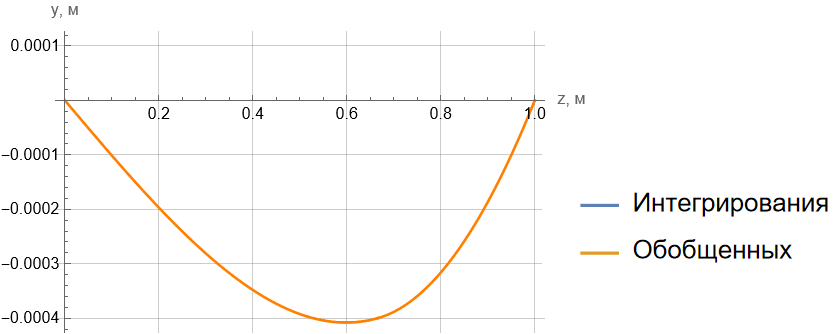
\includegraphics[width=1\textwidth]{g.4}

\end{frame}

\begin{frame}{Результаты}
	В ходе работы получены следующие результаты:
	\begin{block}{}
	\begin{enumerate}
		\item Изучены методы интегрирования и обобщенных функций нахождения уравнения упругого изгиба стержня.	
		\item Решены два типа задач с помощью этих методов, их результаты оказались идентичны.
		\item Метод интегрирования является более трудоемким и менее удобным по сравнению с методом обобщенных функций, так как требует учета большего количества граничных условий и большего объема вычислений.
	\end{enumerate}
	\end{block}	
\end{frame}	
\end{document} 